\chapter{Wasserstoffatom\label{chapter:wasserstoff}}
\lhead{Wasserstoffatom}
\rhead{}
Der bisher entwickelte Formalismus erlaubt bereits, das Wasserstoff-Atom
zu verstehen. Die Quantenmechanik erkl"art die Stabilit"at der
Materie, und sagt das Wasserstoff-Spektrum korrekt voraus.
\section{Schr"odinger-Gleichung f"ur das Wasserstoffatom}
\rhead{Schr"odingergleichung f"ur das Wasserstoffatom}
Die Hamilton-Funktion eines Elektrons im Potential eines einzelnen
Protons, welches sich im Nullpunkt des Koordinatensystems befindet,
ist
\begin{equation}
H=\frac1{2m_e}p^2 + V(r)
=\frac1{2m_e}p^2 - \frac1{4\pi\varepsilon_0}\frac{e^2}{r}.
\label{skript:h2hamilton}
\end{equation}
Darin ist $m_e$ die Masse des Elektrons, $e$ ist die Elementarladung.
$r$ ist die Entfernung eines Punktes vom Nullpunkt.
Der Impuls ist als Vektor zu verstehen, also $p^2=p_x^2+p_y^2+p_z^2$.

Wir suchen eine L"osung des quantisierten Systems mit Zustandsvektoren, die von
den Ortskoordinaten abh"angen.
Nach den Quantisierungsregeln m"ussen die Impulse in der Hamiltonfunktion
durch Ableitungsoperatoren
\begin{equation}
p_x\rightarrow \frac{\hbar}{i}\frac{\partial}{\partial x},
\qquad
p_y\rightarrow \frac{\hbar}{i}\frac{\partial}{\partial y},
\quad
\text{und}
\quad
p_y\rightarrow \frac{\hbar}{i}\frac{\partial}{\partial z}.
\label{skript:h2quant}
\end{equation}
ersetzt werden. Wendet man die Ersetzungen (\ref{skript:h2quant}) auf die
Hamilton-Funktion (\ref{skript:h2hamilton}) an, erh"alt man den Hamilton-Operator
f"ur das Wasserstoff-Atom:
\[
\hat H=-\frac{\hbar^2}{2m_e}\biggl(
\frac{\partial^2}{\partial x^2}+
\frac{\partial^2}{\partial y^2}+
\frac{\partial^2}{\partial z^2}
\biggr)-\frac1{4\pi\varepsilon_0}\frac{e^2}{r}
=-\frac{\hbar^2}{2m_e}\Delta -\frac1{4\pi\varepsilon_0}\frac{e^2}{r}.
\]
Wir suchen zeitunabh"angige Zust"ande, also Eigenfunktionen dieses
Operators. Wir erwarten eine Menge von Zustandsvektoren $|\psi\rangle$
mit zugeh"origen Eigenwerten $E$, so dass
\begin{equation}
\hat H\,|\psi\rangle = E\,|\psi\rangle.
\label{skript:h2schroedinger}
\end{equation}
(\ref{skript:h2schroedinger}) ist eine partielle Differentialgleichung.
Wir beabsichtigen nicht, eine allgemeine Theorie der partiellen
Differentialgleichungen zu entwickeln.
F"ur unsere Zwecke reicht es, eine ad hoc L"osung zu finden.

\section{Kugelkoordinaten}
\rhead{Kugelkoordinaten}
Das Eigenwertproblem (\ref{skript:h2schroedinger}) kann in kartesischen Koordinaten
nicht direkt gel"ost werden. Dies liegt daran, dass die kartesischen
Koordinaten die vorhandene Kugelsymmetrie des Problems nicht ausreichend
ber"ucksichtigen. Es ist viel besser, Kugelkoordinaten zu verwenden.

Die Umrechnungn zwischen Kugelkoordinaten $(r,\vartheta,\varphi)$ und
kartesischen Koordinaten $(x,y,z)$ ist gegeben durch
\begin{align*}
x&=r
\sin\vartheta
\cos\varphi
\\
y&=r
\sin\vartheta
\sin\varphi
\\
z&=r\cos \vartheta
\end{align*}
Eine etwas m"uhsame, im Anhang (Kapitel~\ref{chapter:kugelkoordinaten})
durchgef"uhrte Rechnung erlaubt, den Laplace-Operator in Kugelkoordinaten
auszudr"ucken:
\[
\Delta
=
\frac1{r^2}\frac{\partial}{\partial r}\biggl(
r^2\frac{\partial}{\partial r}
\biggr)
+\frac1{r^2\sin\vartheta}\frac{\partial}{\partial \vartheta}\biggl(
 \sin\vartheta \frac{\partial}{\partial\vartheta}
\biggr)
+
\frac1{r^2\sin^2\vartheta}\frac{\partial^2}{\partial\varphi^2}.
\]

\section{L"osung der Schr"odingergleichung}
\rhead{L"osung der Schr"odingergleichung}
Wir suchen jetzt also L"osungen des Eigenwertproblems (\ref{skript:h2schroedinger})
als $L^2$-Funktionen in Kugel-Koordinaten $(r,\varphi,\vartheta)$. Wir
verwenden dazu die Methode der Separation der Variablen.

\subsection{Separationsansatz}
Wir nehmen an,
dass sich die L"osung $\psi(r,\vartheta,\varphi)$ schreiben l"asst als
ein Produkt von drei Funktionen, die je nur von einer Koordinate
abh"angen. Wir setzen also an
\begin{equation}
\psi(r,\vartheta,\varphi)=R(r)\cdot
\Theta(\vartheta)\cdot
\Phi(\varphi)
\label{skript:sepansatz}
\end{equation}
und setzen dies in das Eigenwertproblem ein. Dazu brauchen wir die Ableitung
nach $r$, $\varphi$ und $\vartheta$ von $\psi(r,\varphi,\vartheta)$, doch
diese Ableitungen wirken jeweils nur auf einen der Faktoren:
\[
\frac{\partial}{\partial r}\psi(r,\vartheta,\varphi)
=
\frac{\partial R(r)}{\partial r}
\cdot \Theta(\vartheta)
\cdot  \Phi(\varphi)
+
R(r)
\cdot \Theta(\vartheta)
\cdot \underbrace{\frac{\partial\Phi(\varphi)}{\partial r}}_{=0}
+
R(r)
\cdot \underbrace{\frac{\partial \Theta(\vartheta)}{\partial r}}_{=0}
\cdot \Phi(\varphi)
=
R'(r)
\cdot \Theta(\vartheta),
\cdot \Phi(\varphi)
\]
und analog f"ur die anderen Variablen.
Wir k"onnen also so tun, als ob die Ableitungen jeweils nur auf genau
einen der Faktoren wirken.
\begin{equation}
\Delta \psi
=
\frac1{r^2}\frac{d}{dr}\bigl(r^2R'(r)\bigr)
\cdot \Theta(\vartheta)
\cdot \Phi(\varphi)
+
R(r)
\cdot \frac{1}{r^2\sin\vartheta}
\frac{d}{d\vartheta}(\sin\vartheta \Theta'(\vartheta))
\cdot \Phi(\varphi)
+
\frac{R(r)}{r^2\sin^2\vartheta}
\cdot \Theta(\vartheta)
\cdot \Phi''(\varphi)
\label{skript:separated}
\end{equation}
Man beachte, dass in allen Termen immer nur einer der Faktoren des
Separationsansatzes abgeleitet wurde.

Das Eigenwertproblem, welches zu l"osen ist, wird jetzt in Kugelkoordinaten
zu
\[
-\frac{\hbar^2}{2m_e} \Delta\psi(r,\vartheta,\varphi)
-\frac{1}{4\pi\varepsilon_0}\frac{e^2}{r}\psi(r,\vartheta,\varphi)
=E\psi(r,\vartheta,\varphi).
\]

\subsection{Separation von $\varphi$}
Keine der drei Faktoren des Ansatzes (\ref{skript:sepansatz}) f"ur
$\psi(r,\vartheta,\varphi)$ kann verschwinden, sonst erhielten wir die 
Nullfunktion, also nicht einen Eigenvektor von $\hat H$.
Nat"urlich k"onnen die Faktoren einzelne Nullstellen haben, aber ausserhalb
dieser Nullstellen kann man die Gleichung (\ref{skript:separated}) durch 
$\psi(r,\vartheta,\varphi)$ teilen. Wir erhalten
\begin{equation*}
-\frac{\hbar^2}{2m_e}\biggl(
\frac{1}{R(r)}
\frac{1}{r^2}
\frac{d}{dr}(r^2R'(r))
+
\frac{1}{\Theta(\vartheta) r^2\sin\vartheta}\frac{d}{d\vartheta}(\sin\vartheta \Theta'(\vartheta))
+
\frac{1}{r^2\sin^2\vartheta}\frac{\Phi''(\varphi)}{\Phi(\varphi)}
\biggr)
-\frac1{4\pi\varepsilon_0}\frac{e^2}{r}
=
E.
\end{equation*}
Bringen wir ausserdem alle Terme mit $\varphi$ auf die rechte Seite,
und multiplizieren mit $r^2\sin^2\vartheta$
ergibt sich
\begin{equation*}
-\frac{\hbar^2}{2m_e}
\frac{1}{R(r)}\sin^2\vartheta \frac{d}{dr}(r^2R'(r))
-
\frac{\hbar^2}{2m_e}
\frac{\sin\vartheta}{\Theta(\vartheta) }\frac{d}{d\vartheta}(\sin\vartheta \Theta'(\vartheta))
-\biggl(\frac1{4\pi\varepsilon_0}\frac{e^2}{r}
+
E\biggr)r^2\sin^2\vartheta
=
\frac{\hbar^2}{2m_e}\frac{\Phi''(\varphi)}{\Phi(\varphi)}.
\end{equation*}
Indem wir durch den Faktor $-\hbar^2/2m_e$ dividieren, wir die Gleichung
etwas "ubersichtlicher:
\begin{equation}
\frac{1}{R(r)}\sin^2\vartheta \frac{d}{dr}(r^2R'(r))
+
\frac{\sin\vartheta}{\Theta(\vartheta) }\frac{d}{d\vartheta}(\sin\vartheta \Theta'(\vartheta))
+\biggl(\frac{m_e}{2\pi\varepsilon_0\hbar^2}\frac{e^2}{r}
+
\frac{2m_eE}{\hbar^2}\biggr)r^2\sin^2\vartheta
=
-\frac{\Phi''(\varphi)}{\Phi(\varphi)}.
\label{skript:phisepariert}
\end{equation}
Die linke Seite dieser Gleichung h"angt nicht von $\varphi$ ab, also
darf auch die rechte Seite nicht von $\varphi$ abh"angen, sie muss
eine Konstante sein. Wir nennen die Konstante $m^2$ (dies wird sich
als zweckm"assig herausstellen). Wir haben also aus der urspr"unglichen
partiellen Differentialgleichung eine gew"ohnliche Differentialgleichung
\[
-\frac{\Phi''(\varphi)}{\Phi(\varphi)}=m^2
\quad\Leftrightarrow\quad
\Phi''(\varphi)=-m^2\Phi(\varphi)
\]
f"ur die Funktion $\Phi(\varphi)$ gefunden.
Die L"osungen einer solchen Differentialgleichung zweiter Ordnung sind
wohl bekannt: $e^{im\varphi}$ und $e^{-im\varphi}$. Damit die Funktion
periodisch wird, muss $m$ eine nat"urliche Zahl sein, $m=0,1,2,\dots$.

\subsection{Separation von $r$ und $\vartheta$}
In der Gleichung (\ref{skript:phisepariert}) kommt auf der linken Seite nur
noch $r$ und $\vartheta$ vor.  Die rechte Seite haben wir inzwischen auf
die m"oglichen Werte $m^2$ reduziert. Teilen wir die Gleichung durch
$\sin^2\vartheta$, und bringen die von $\vartheta$ abh"angenden Terme
auf die rechte Seite, erhalten wir die Gleichung
\begin{equation}
\frac{1}{R(r)}\frac{d}{dr}\bigl(r^2R'(r)\bigr)
+\biggl(\frac{m_e}{2\pi\varepsilon_0\hbar^2}\frac{e^2}{r}
+
\frac{2m_eE}{\hbar^2}\biggr)r^2
=
-
\frac1{\sin\vartheta\Theta(\vartheta) }
\frac{d}{d\vartheta}\bigl(\sin\vartheta \Theta'(\vartheta)\bigr)
+
\frac{m^2}{\sin^2\vartheta}
\label{skript:thetasepariert}
\end{equation}
Die linke Seite von (\ref{skript:thetasepariert}) h"angt nicht von $\vartheta$
ab, also kann auch die rechte Seite nicht von $\vartheta$ abh"angen.
Ebenso h"angt die rechte Seite nicht von $r$, also kann auch die linke
nicht von $r$ abh"angen. Beide Seiten m"ussen also konstant sein,
wir nennen die Konstante $\lambda$.

\subsection{Abh"angigkeit von $\vartheta$}
Die Funktion $\Theta(\vartheta)$ auf der rechten Seite ist eigentlich
eine Funktion von $z=\cos\vartheta$. Wir schreiben
$Z(z)=Z(\cos\vartheta)=\Theta(\vartheta)$. Die Ableitung nach $\vartheta$
kann dann umgeschrieben werden in eine Ableitung nach $z$
\begin{align*}
\Theta'(\vartheta)&=
\frac{d}{d\vartheta}Z(z)=Z'(z)\frac{dz}{d\vartheta}=-\sin\vartheta Z'(z)
\\
\frac{d}{dz}
&=
-\frac1{\sin\vartheta}\frac{d}{d\vartheta}
\end{align*}
Nat"urlich gilt auch $1-z^2=\sin^2\vartheta$, so dass die rechte Seite
von (\ref{skript:thetasepariert}) zu
\begin{equation}
-
\frac1{\Theta(\vartheta)}
\frac1{\sin\vartheta}
\frac{d}{d\vartheta}\biggl(
\sin^2\vartheta \frac1{\sin\vartheta}\frac{d}{d\vartheta}\Theta'(\vartheta)
\biggr)
+
\frac{m^2}{\sin^2\vartheta}
=
-\frac1{Z(z)}\frac{d}{dz}\biggl(
(1-z^2)\frac{d}{dz}Z(z)
\biggr)
+
\frac{m^2}{1-z^2}
\end{equation}
wird. Dieser Ausdruck muss konstant sein, wir nennen die Konstante 
$\lambda$:
\begin{equation}
-\frac1{Z(z)}\frac{d}{dz}\biggl(
(1-z^2)\frac{d}{dz}Z(z)
\biggr)
+
\frac{m^2}{1-z^2}
=\lambda
\end{equation}
oder
\begin{equation}
\frac{d}{dz}\biggl(
(1-z^2)\frac{d}{dz}Z(z)
\biggr)
+\biggl(\lambda
-
\frac{m^2}{1-z^2}
\biggr)Z(z)
=0
\label{skript:legendregleichung}
\end{equation}

\subsubsection{Spezialfall $m=0$}
Wir untersuchen diese L"osung zun"achst f"ur den Spezialfall $m=0$,
d.~h.~wir m"ussen die Differentialgleichung
\begin{equation}
\frac{d}{dz}\biggl(
(1-z^2)\frac{d}{dz}Z(z)
\biggr)
+\lambda Z(z)=0
\label{skript:Zequation}
\end{equation}
l"osen.
Dies ist die sogenannte Legendresche Differentialgleichung,
deren L"osung in einer guten Formelsammlung gefunden werden k"onnen.

Wir versuchen eine L"osung in Form eines Polynoms vom
Grade $l$ zu finden, also 
\begin{equation}
P_l(z)=a_0+a_1z+\dots+a_lz^l.
\label{skript:legendreansatz}
\end{equation}
Setzen wir dies in die Gleichung~(\ref{skript:Zequation}) ein, und betrachten nur die
Terme vom Grad $z^l$:
\begin{align*}
\frac{d}{dz}(-z^2la_lz^{l-1})
+
\lambda a_lz^l&=0
\\
-l(l+1)a_lz^l+\lambda a_lz^l&=0,
\end{align*}
Es folgt, dass $\lambda = l(l+1)$ sein muss, wobei $l$ eine ganze
Zahl sein muss.

Wie jede Differentialgleichung zweiter Ordnung hat die Legendresche
Differentialgleichung ausser den $P_l$ auch noch eine L"osung
$Q_l$, diese ist jedoch nicht eschr"ankt und kommt daher als L"osungsfunktion
f"ur unser Problem nicht in Frage.

\subsubsection{Legendre-Polynome}
Indem man den Ansatz (\ref{skript:legendreansatz}) f"ur alle Koeffizienten
auswertet, nicht nur f"ur $a_l$, kann man die Polynome $P_l(z)$ 
bestimmen, sie heissen Legendre-Polynome.
"Uber die Jahre wurde eine umfangreiche Theorie der Legendre-Polynome
aufgebaut, so gilt zum Beispiel die folgende Formel von Rodrigues
\[
P_l(z)=\frac1{2^ll!}\frac{d^l}{dz^l}(z^2 - 1)^l.
\]
Die Legendre-Polynome sind orthogonal.

%Durch Einsetzen in die Differentialgleichung kann man verifizieren,
%dass dies tats"achlich eine L"osung ist:
%\begin{align*}
%\frac{d}{dz}\biggl(
%(1-z^2)\frac{d}{dz}
%\frac1{2^ll!}\frac{d^l}{dz^l}(z^2 - 1)^l.
%\biggr)
%&=
%\frac1{2^ll!}
%\frac{d}{dz}\biggl(
%(1-z^2)
%\frac{d^l}{dz^l}l(z^2 - 1)^{l-1}2z.
%\biggr)
%\\
%&=
%\frac1{2^ll!}
%\biggl(
%(-2z)
%\frac{d^l}{dz^l}l(z^2 - 1)^{l-1}2z.
%+
%(1-z^2)
%\frac{d^l}{dz^l}l\frac{d}{dz}\bigl((z^2 - 1)^{l-1}2z\bigr)
%\biggr)
%\\
%\end{align*}

\subsubsection{Der Fall $m\ne 0$}
F"ur den allgemeinen Fall mit beliebigen $m$ m"ussen L"osungen der
Gleichung
\begin{equation}
\frac{d}{dz}\biggl((1-z^2)\frac{d}{dz}Z(z)\biggr)
+\biggl(\lambda -\frac{m^2}{1-z^2}\biggr)Z(z)=0
\end{equation}
gefunden werden. Man kann zeigen, dass die Funktionen
\[
P_l^m(z)=
(1-z^2)^{\frac{m}2}\frac{d^m}{dz^m}P_l(z)
\]
eine L"osung f"ur $\lambda=l(l+1)$ ist.
Auch diese allgemeineren Funktionen $P_l^m(z)$ sind orthogonal.

\subsection{Abh"angigkeit von $r$}
Die Funktion $R(r)$ erf"ullt die Differentialgleichung
\begin{align}
\frac{1}{r^2}\frac{d}{dr}\bigl(r^2R'(r)\bigr)
+\biggl(\frac{m_e}{2\pi\varepsilon_0\hbar^2}\frac{e^2}{r}
+
\frac{2m_eE}{\hbar^2}
-\frac{\lambda}{r^2}
\biggr)R(r)
&=0
\label{skript:radialgleichung}
\end{align}
\begin{figure}
\centering
\includegraphics{graphics/h-1.pdf}
\caption{Durch den Drehimpuls modifiziertes effektives Potential.
\label{skript:modifiziertes-potential}}
\end{figure}
Wir wissen bereits, dass $\lambda=l(l+1)$, also k"onnen wir die
Gleichung umformen zu
\begin{align*}
\frac{1}{r^2}\frac{d}{dr}\bigl(r^2R'(r)\bigr)
+\biggl(\frac{m_e}{2\pi\varepsilon_0\hbar^2}\frac{e^2}{r}
+
\frac{2m_eE}{\hbar^2}
-\frac{l(l+1)}{r^2}
\biggr)R(r)
&=0.
\end{align*}
Der Drehimpuls $l$ modifiziert das Potential mit einem Term
$\sim\frac1{r^2}$ (Abbildung~\ref{skript:modifiziertes-potential}).

Die Gleichungen k"onnen etwas vereinfacht werden, wenn man einen
Faktor $r$ abspaltet, also 
\[
R(r)=\frac{\chi(r)}{r}
\]
verwendet.
Die Ableitungen von $R(r)$ sind
\begin{align*}
R'(r)&=\frac{\chi'(r)r-\chi(r)}{r^2},\\
\frac{d}{dr}\bigl(r^2R'(r)\bigr)
&=
\frac{d}{dr}\bigl(\chi'(r)r-\chi(r)\bigr)
=
\chi''(r)r+\chi'(r)-\chi'(r)=r\chi''(r).
\end{align*}
Setzt man dies in die Differentialgleichung (\ref{skript:radialgleichung}) ein,
erh"alt
\begin{align*}
\frac{\chi''(r)}{r}
+\biggl(\frac{m_e}{2\pi\varepsilon_0\hbar^2}\frac{e^2}{r}
+
\frac{2m_eE}{\hbar^2}
-\frac{l(l+1)}{r^2}
\biggr)\frac{\chi(r)}{r}
&=0
\\
\chi''(r)
+\biggl(\frac{m_e}{2\pi\varepsilon_0\hbar^2}\frac{e^2}{r}
+
\frac{2m_eE}{\hbar^2}
-\frac{l(l+1)}{r^2}
\biggr)\chi(r)
&=0
\end{align*}


Die gesuchte L"osung $R(r)$ muss f"ur grosse Entfernungen $r$ exponentiell
abfallen.
Wir versuchen daher einen Ansatz der Form
\[
R(r)=\biggl(\frac{2r}{n}\biggr)^le^{-\frac{r}{n}}w\biggl(\frac{2r}{n}\biggr)
\]

%Wir versuchen eine L"osung f"ur $R(r)$ zu finden. Um die Differentialgleichung
%f"ur $R(r)$ etwas zu vereinfachen, formulieren wir sie um f"ur 
%\[
%R(r)=\frac{\chi(r)}{r}.
%\]
%Die Ableitung von $R(r)$ ist
%\[
%R'(r)=\frac{\chi'(r)r-\chi(r)}{r^2},
%\]
%Der erste Term in (\ref{skript:thetasepariert}) wird dadurch besonders einfach,
%n"amlich
%\[
%\frac1{r^2}\frac{d}{dr}\bigl(r^2R'(r)\bigr)
%=\frac1{r^2}\frac{d}{dr} \bigl(\chi'(r)r-\chi(r)\bigr)
%=\frac1{r^2}(\chi''(r)r +\chi'(r) -\chi'(r))=\frac{\chi''(r)}r,
%\]
%und die Differentialgleichung wird
%\begin{align*}
%\frac{\chi''(r)}{r}
%+
%\biggl(\frac{m_e}{2\pi\varepsilon_0\hbar^2}\frac{e^2}{r}
%+
%\frac{2m_eE}{\hbar^2}
%-\frac{\lambda}{r^2}
%\biggr)R(r)
%&=0
%\\
%\Rightarrow\qquad
%\chi''(r)
%+
%\biggl(\frac{m_e}{2\pi\varepsilon_0\hbar^2}\frac{e^2}{r}
%+
%\frac{2m_eE}{\hbar^2}
%-\frac{\lambda}{r^2}
%\biggr)\chi(r)
%&=0.
%\end{align*}

\begin{figure}
\centering
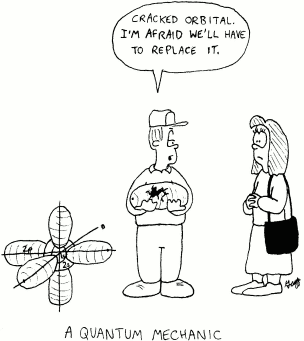
\includegraphics[width=0.4\hsize]{images/crackedorbital.png}
\caption{Berufsbild des Quantenmechanikers: Kenntnisse der Orbitale
sind unerl"asslich\label{skript:crackedorbital}}
\end{figure}

\section{Hybridorbitale}
